\documentclass[11pt]{beamer}

\usecolortheme[light,accent=blue]{solarized}
\setbeamercovered{transparent=0}
\setbeamertemplate{navigation symbols}{} % remove navigation symbols
\setbeamertemplate{section in toc}[sections numbered] % numbered sections
% \setbeamertemplate{footline}[page number]
\setbeamertemplate{footline}{
  \hfill%
  \usebeamercolor[fg]{page number in head/foot}%
  \usebeamerfont{page number in head/foot}%
  \setbeamertemplate{page number in head/foot}[framenumber]%
  \usebeamertemplate*{page number in head/foot}\kern1em\vskip2pt%
}
\setbeamerfont{page number in head/foot}{size=\small}
\setbeamerfont{note page}{size=\scriptsize}
\addtobeamertemplate{note page}{\setbeamerfont{itemize/enumerate subbody}{size=\tiny}}{}
\setbeamertemplate{bibliography item}{\insertbiblabel}

\usepackage[english]{babel}
\usepackage{amsmath,amssymb}
\usepackage{physics}
\usepackage{tikz}
\usepackage{listings}

%%%%%%%%%%%%%%%%%%%%%%%%%%%%%%%%%%%%%%%%%%%%%%%%%%

\usetikzlibrary{calc,decorations.markings,decorations.pathmorphing,positioning,shapes,scopes}

\tikzset{
  >=latex,
  ->-/.style={postaction={decorate},decoration={%
      markings,mark=at position #1 with {\arrow{>}}%
    }%
  },%
  ->-/.default=.5,
  -<-/.style={postaction={decorate},decoration={%
      markings,mark=at position #1 with {\arrowreversed{>}}%
    }%
  },%
  -<-/.default=.5,
}

\tikzstyle{block} = [rectangle, draw, text width=7em, text centered, minimum height=2em]

\lstset{
  backgroundcolor=\color{white},   % choose the background color; you must add \usepackage{color} or \usepackage{xcolor}; should come as last argument
  basicstyle=\footnotesize\ttfamily,        % the size of the fonts that are used for the code
  breaklines=true,                 % sets automatic line breaking
  stepnumber=1,
  prebreak=\textbackslash,
  commentstyle=\color{gray},       % comment style
  % deletekeywords={...},            % if you want to delete keywords from the given language
  % escapeinside={\%*}{*)},          % if you want to add LaTeX within your code
  % extendedchars=true,              % lets you use non-ASCII characters; for 8-bits encodings only, does not work with UTF-8
  frame=single,	                   % adds a frame around the code
  keepspaces=true,                 % keeps spaces in text, useful for keeping indentation of code (possibly needs columns=flexible)
  keywordstyle=\color{blue},       % keyword style
  morekeywords={wget},             % if you want to add more keywords to the set
  numbers=left,                    % where to put the line-numbers; possible values are (none, left, right)
  numbersep=5pt,                   % how far the line-numbers are from the code
  numberstyle=\tiny\color{gray},   % the style that is used for the line-numbers
  rulecolor=\color{gray},         % if not set, the frame-color may be changed on line-breaks within not-black text (e.g. comments (green here))
  showspaces=false,                % show spaces everywhere adding particular underscores; it overrides 'showstringspaces'
  showstringspaces=false,          % underline spaces within strings only
  showtabs=false,                  % show tabs within strings adding particular underscores
  % stringstyle=\color{red},         % string literal style
  tabsize=2,	                   % sets default tabsize to 2 spaces
}

\newcommand{\CXX}{\texttt{C++}}
\newcommand{\CalcHEP}{\texttt{CalcHEP}}
\newcommand{\FORTRAN}{\texttt{FORTRAN}}
\newcommand{\FlexibleSUSY}{\texttt{FlexibleSUSY}}
\newcommand{\HiggsTools}{\texttt{HiggsTools}}
\newcommand{\ii}{\text{i}}
\newcommand{\hc}{\text{h.c.}}
\newcommand{\Lagr}{\mathcal{L}}
\newcommand{\Lagrin}{\mathcal{L}_{\text{int}}}
\newcommand{\LoopTools}{\texttt{LoopTools}}
\newcommand{\Mathematica}{\texttt{Mathematica}}
\newcommand{\micrOMEGAs}{\texttt{micrOMEGAs}}
\newcommand{\SARAH}{\texttt{SARAH}}
\newcommand{\SESM}{\text{SESM}}
\newcommand{\SM}{\text{SM}}
\newcommand{\SPheno}{\texttt{SPheno}}
\newcommand{\TSESM}{\text{TSESM}}

%%%%%%%%%%%%%%%%%%%%%%%%%%%%%%%%%%%%%%%%%%%%%%%%%%

\definecolor{red}{rgb}{1.0,0.2,0.2}
\definecolor{blue}{rgb}{0,0.7,1.0}
\definecolor{green}{rgb}{0,1.0,0.5}

%%%%%%%%%%%%%%%%%%%%%%%%%%%%%%%%%%%%%%%%%%%%%%%%%%

\title{Tools for HEP}
\subtitle{From $\Lagr$ to Observables}

\author[Voigt]{Alexander Voigt\\ \href{mailto://alexander.voigt@physik.rwth-aachen.de}{alexander.voigt@physik.rwth-aachen.de}}
\institute[RWTH Aachen]{RWTH Aachen}
\date{Workshop on\\ ``Selected topics on future directions in particle physics''\\ Warsaw 2024}

\begin{document}

%%%%%%%%%%%%%%%%%%%%%%%%%%%%%%%%%%%%%%%%%%%%%%%%%%

\begin{frame}
  \titlepage
\end{frame}

%%%%%%%%%%%%%%%%%%%%%%%%%%%%%%%%%%%%%%%%%%%%%%%%%%

\begin{frame}{Table of Contents}
  \tableofcontents
\end{frame}

%%%%%%%%%%%%%%%%%%%%%%%%%%%%%%%%%%%%%%%%%%%%%%%%%%

\section{Overview}

\begin{frame}{Overview}
  \begin{center}
    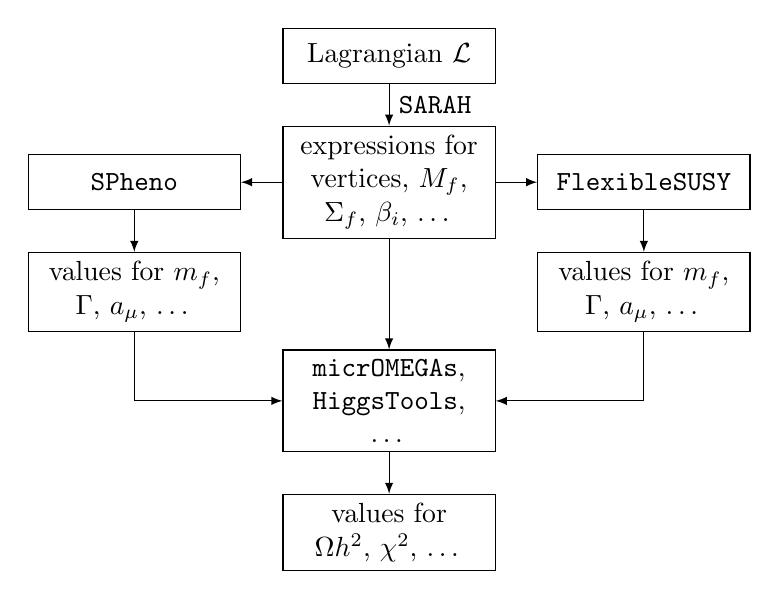
\begin{tikzpicture}[node distance=1.5em, auto]
      \node[block] (L) { Lagrangian $\Lagr$ };
      \node[block, below=of L] (E) { expressions for vertices, $M_f$, $\Sigma_f$, $\beta_i$, \ldots };
      \node[block, left=of E] (S) { \SPheno };
      \node[block, below=of S] (SO) { values for $m_f$, $\Gamma$, $a_\mu$, \ldots };
      \node[block, right=of E] (F) { \FlexibleSUSY };
      \node[block, below=of F] (FO) { values for $m_f$, $\Gamma$, $a_\mu$, \ldots };
      \node[block, below=4em of E] (O) { \micrOMEGAs, \HiggsTools, \ldots };
      \node[block, below=of O] (O2) { values for $\Omega h^2$, $\chi^2$, \ldots };
      \draw[->] (L) -- node[right] { \SARAH } (E);
      \draw[->] (E) -- (S);
      \draw[->] (E) -- (F);
      \draw[->] (S) -- (SO);
      \draw[->] (F) -- (FO);
      \draw[->] (SO) |- (O);
      \draw[->] (FO) |- (O);
      \draw[->] (E) -- (O);
      \draw[->] (O) -- (O2);
    \end{tikzpicture}
  \end{center}
\end{frame}

%%%%%%%%%%%%%%%%%%%%%%%%%%%%%%%%%%%%%%%%%%%%%%%%%%

\section{Standard Model}

%%%%%%%%%%%%%%%%%%%%%%%%%%%%%%%%%%%%%%%%%%%%%%%%%%

\begin{frame}{Table of Contents}
  \tableofcontents[currentsection]
\end{frame}

%%%%%%%%%%%%%%%%%%%%%%%%%%%%%%%%%%%%%%%%%%%%%%%%%%

\begin{frame}[fragile]{\insertsection\ -- What we will do}
  \begin{enumerate}
  \item Inspect the \SARAH\ model files and generate some analytic
    expressions
  \item Create a \SPheno\ spectrum generator
  \item Create a \FlexibleSUSY\ spectrum generator
  \end{enumerate}
\end{frame}

%%%%%%%%%%%%%%%%%%%%%%%%%%%%%%%%%%%%%%%%%%%%%%%%%%

\subsection{SARAH}

%%%%%%%%%%%%%%%%%%%%%%%%%%%%%%%%%%%%%%%%%%%%%%%%%%

\begin{frame}{Table of Contents}
  \tableofcontents[currentsection,currentsubsection]
\end{frame}

%%%%%%%%%%%%%%%%%%%%%%%%%%%%%%%%%%%%%%%%%%%%%%%%%%

\begin{frame}[fragile]{\insertsection\ -- SARAH -- inspect model files}

  Go to the \SARAH\ directory:
  %
  \begin{lstlisting}
$ cd ~/hep-software/SARAH\end{lstlisting}%$
  %
  Let's inspect the following \SARAH\ files:
  \begin{itemize}
  \item \texttt{Models/SM/SM.m}\\ Definitions of the gauge
    group, fields, Lagrangian, VEVs, field mixings, \ldots
  \item \texttt{Models/SM/particles.m}\\
    Definitions of properties of the fields (output name, \LaTeX\
    name, PDG number, FeynArts number, \ldots)
  \item \texttt{Models/SM/parameters.m}\\
    Definitions of information about the model parameters (Output
    name, \LaTeX\ name, SLHA output block, \ldots)
  \end{itemize}

  \bigskip

  References: \url{https://sarah.hepforge.org/}
\end{frame}

%%%%%%%%%%%%%%%%%%%%%%%%%%%%%%%%%%%%%%%%%%%%%%%%%%

\begin{frame}[fragile]{\insertsection\ -- SARAH -- inspect model properties}
  Let's start \SARAH\ and inspect some model properties.

  \medskip

%   Go to \texttt{$\sim$/hep-software/SARAH}:
%   \begin{lstlisting}
% $ cd ~/hep-software/SARAH\end{lstlisting}%$
  %
  Start \Mathematica:
  \begin{lstlisting}
$ math\end{lstlisting}%$
  %
  Run
  %
  \begin{lstlisting}
In[]:= << SARAH`
In[]:= << Start["SM"]
In[]:= SARAH`Commands (* shows available commands *)\end{lstlisting}
  %
  Let's inspect some model properties:
  %
  \begin{lstlisting}
In[]:= SARAHparameters (* parameters *)
In[]:= Particles[EWSB] (* fields after EWSB *)
In[]:= MassMatrix[Fe]  (* mass matrix of Fe *)
In[]:= Vertex[{bar[Fe],Fe,VP}] (* a vertex *)\end{lstlisting}
\end{frame}

%%%%%%%%%%%%%%%%%%%%%%%%%%%%%%%%%%%%%%%%%%%%%%%%%%

\begin{frame}[fragile]{\insertsection\ -- SARAH -- generate some expressions}
  Let's  generate some analytic expressions.
  %
  \begin{lstlisting}
In[]:= MakeAll[] (* generate all expressions *)
In[]:= Quit[] (* quit *)\end{lstlisting}
  %
  The expressions are written to the \texttt{Output/SM/} sub-directory.

  \medskip

  Vertices (fermion--fermion--gauge boson):
  %
  \begin{lstlisting}
$ less Output/SM/EWSB/Vertices/VertexListFFV.m\end{lstlisting}%$
  %
  Beta functions (gauge couplings):
  %
  \begin{lstlisting}
$ less Output/SM/RGEs/BetaGauge.m\end{lstlisting}%$
  %
  1-loop self-energies:
  %
  \begin{lstlisting}
$ less Output/SM/EWSB/One-Loop/SelfEnergy.m\end{lstlisting}%$
\end{frame}

%%%%%%%%%%%%%%%%%%%%%%%%%%%%%%%%%%%%%%%%%%%%%%%%%%

\subsection{SPheno}

%%%%%%%%%%%%%%%%%%%%%%%%%%%%%%%%%%%%%%%%%%%%%%%%%%

\begin{frame}{Table of Contents}
  \tableofcontents[currentsection,currentsubsection]
\end{frame}

%%%%%%%%%%%%%%%%%%%%%%%%%%%%%%%%%%%%%%%%%%%%%%%%%%

\begin{frame}[fragile]{\insertsection\ -- SPheno -- spectrum generator}
  Let's create a \SPheno\ spectrum generator for the SM.

  \bigskip

  Let's first look into the \SPheno\ model file for the SM:
  %
  \begin{lstlisting}
$ less Models/SM/SPheno.m\end{lstlisting}%$
  %
  It defines boundary conditions for input and output parameters, loop
  corrections, observables, \ldots

  \bigskip

  Now we'll create the FORTRAN source code for the \SPheno\ spectrum
  generator:
  %
  \begin{lstlisting}
$ math
In[]:= << SARAH`
In[]:= Start["SM"]
In[]:= MakeSPheno[]
In[]:= Quit[]\end{lstlisting}%$

\end{frame}

%%%%%%%%%%%%%%%%%%%%%%%%%%%%%%%%%%%%%%%%%%%%%%%%%%

\begin{frame}[fragile]{\insertsection\ -- SPheno -- spectrum generator}
  Now go to the \SPheno\ directory and copy the generated FORTRAN
  files to the \SM\ sub-directory.
  %
  \begin{lstlisting}
$ cd ~/hep-software/SPheno-4.0.5
$ mv ~/hep-software/SARAH/Output/SM/EWSB/SPheno SM\end{lstlisting}%$
  %
  Then we compile the source code:
  %
  \begin{lstlisting}
$ make F90=gfortran
$ make F90=gfortran Model=SM\end{lstlisting}%$
  %
  Now we can run the spectrum generator and inspect the SLHA output file:
  %
  \begin{lstlisting}
$ bin/SPhenoSM SM/Input_Files/LesHouches.in.SM
$ less SPheno.spc.SM\end{lstlisting}
\end{frame}

%%%%%%%%%%%%%%%%%%%%%%%%%%%%%%%%%%%%%%%%%%%%%%%%%%

\subsection{FlexibleSUSY}

%%%%%%%%%%%%%%%%%%%%%%%%%%%%%%%%%%%%%%%%%%%%%%%%%%

\begin{frame}{Table of Contents}
  \tableofcontents[currentsection,currentsubsection]
\end{frame}

%%%%%%%%%%%%%%%%%%%%%%%%%%%%%%%%%%%%%%%%%%%%%%%%%%

\begin{frame}[fragile]{\insertsection\ -- FlexibleSUSY -- spectrum generator}
  \begin{center}
    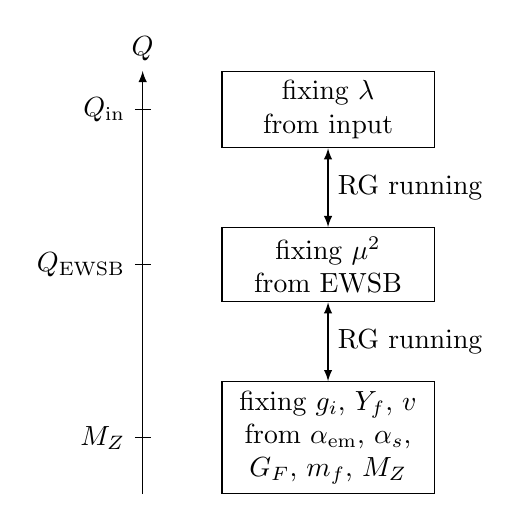
\begin{tikzpicture}
      \pgfmathsetmacro{\Qdist}{1};
      \node[block] (LowScaleInput) { fixing $g_i$, $Y_f$, $v$ from $\alpha_{\text{em}}$, $\alpha_s$, $G_F$, $m_f$, $M_Z$ };
      \node[block,above=1cm of LowScaleInput] (SUSYScaleInput) { fixing $\mu^2$ from EWSB };
      \node[block,above=1cm of SUSYScaleInput] (HighScaleInput) { fixing $\lambda$ from input };
      %
      \draw[<->] (LowScaleInput) -- node[right] {RG running} (SUSYScaleInput);
      \draw[<->] (SUSYScaleInput) -- node[right] {RG running} (HighScaleInput);
      \draw[->] ($(LowScaleInput.south west)+(-\Qdist,0)$) -- ($(HighScaleInput.north west)+(-\Qdist,0)$) node[above] {$Q$};
      \draw[] ($(LowScaleInput.west)+(-1.1*\Qdist,0)$) node[left] {$M_Z$} -- ($(LowScaleInput.west)+(-0.9*\Qdist,0)$);
      \draw[] ($(SUSYScaleInput.west)+(-1.1*\Qdist,0)$) node[left] {$Q_{\text{EWSB}}$} -- ($(SUSYScaleInput.west)+(-0.9*\Qdist,0)$);
      \draw[] ($(HighScaleInput.west)+(-1.1*\Qdist,0)$) node[left] {$Q_{\text{in}}$} -- ($(HighScaleInput.west)+(-0.9*\Qdist,0)$);
    \end{tikzpicture}
  \end{center}
\end{frame}

%%%%%%%%%%%%%%%%%%%%%%%%%%%%%%%%%%%%%%%%%%%%%%%%%%

\begin{frame}[fragile]{\insertsection\ -- FlexibleSUSY -- spectrum generator}
  Let's now create a \FlexibleSUSY\ spectrum generator for the SM.

  \bigskip

  Go into the FlexibleSUSY-2.8.0 directory:
  \begin{lstlisting}
$ cd ~/hep-software/FlexibleSUSY-2.8.0\end{lstlisting}%$
  %
  Let's first look into the \FlexibleSUSY\ model file for the SM:
  %
  \begin{lstlisting}
$ less model_files/SM/FlexibleSUSY.m.in\end{lstlisting}%$
  %
  It defines boundary conditions for input and output parameters, loop
  corrections, observables, \ldots

  \bigskip

  References:\\
  \url{https://arxiv.org/abs/1406.2319}\\
  \url{https://arxiv.org/abs/1710.03760}

\end{frame}

%%%%%%%%%%%%%%%%%%%%%%%%%%%%%%%%%%%%%%%%%%%%%%%%%%

\begin{frame}[fragile]{\insertsection\ -- FlexibleSUSY -- spectrum generator}
  Now we'll build the \FlexibleSUSY\ spectrum generator for the SM.

  \bigskip

  Define a variable to contain the \LoopTools\ directory
  \begin{lstlisting}
$ LT=$HOME/hep-software/LoopTools/build\end{lstlisting}%$
  Create and build the SM spectrum generator:
  \begin{lstlisting}
$ ./createmodel --name=SM
$ ./configure --with-models=SESM \
     --with-loop-libraries=looptools \
     --with-looptools-incdir=${LT}
     --with-looptools-libdir=${LT}
$ make -j4\end{lstlisting}%$
  %
  Run the spectrum generator (set \texttt{FlexibleSUSY[31] = 2}):
  %
  \begin{lstlisting}
$ models/SM/run_SM.x \
    --slha-input-file=models/SM/LesHouches.in.SM\end{lstlisting}%$
\end{frame}

%%%%%%%%%%%%%%%%%%%%%%%%%%%%%%%%%%%%%%%%%%%%%%%%%%

\section{Standard Model + S}

%%%%%%%%%%%%%%%%%%%%%%%%%%%%%%%%%%%%%%%%%%%%%%%%%%

\begin{frame}{Table of Contents}
  \tableofcontents[currentsection]
\end{frame}

%%%%%%%%%%%%%%%%%%%%%%%%%%%%%%%%%%%%%%%%%%%%%%%%%%

\begin{frame}{\insertsection}
  As a second example, let's consider an extension of the SM by an
  extra real scalar gauge singlet. The model should be called Singlet
  Extension of the Standard Model (\SESM).  The Lagrangian should read
  %
  \begin{equation*}
    \Lagr_{\SESM} = \Lagr_{\SM} - \left[\kappa_{SH} H^\dagger H s + \frac{\lambda_{SH}}{2} H^\dagger H s^2 + \frac{M_S^2}{2} s^2 + \frac{\kappa_S}{3} s^3 + \frac{\lambda_S}{2} s^4\right]
  \end{equation*}
  %
  We will proceed as follows:
  %
  \begin{enumerate}
  \item Create a \SARAH\ model file for the SESM
  \item Create a \FlexibleSUSY\ model file for the SESM and run it
  \item Create a \SPheno\ model file for the SESM and run it
  \end{enumerate}
\end{frame}

%%%%%%%%%%%%%%%%%%%%%%%%%%%%%%%%%%%%%%%%%%%%%%%%%%

\subsection{SARAH}

%%%%%%%%%%%%%%%%%%%%%%%%%%%%%%%%%%%%%%%%%%%%%%%%%%

\begin{frame}{Table of Contents}
  \tableofcontents[currentsection,currentsubsection]
\end{frame}

%%%%%%%%%%%%%%%%%%%%%%%%%%%%%%%%%%%%%%%%%%%%%%%%%%

\begin{frame}[fragile]{\insertsection\ -- SARAH -- model file}
  First, we will create a \SARAH\ model file for our new SESM model.

  \bigskip

  Go into the \SARAH\ directory:
  %
  \begin{lstlisting}
$ cd ~/hep-software/SARAH\end{lstlisting}%$
  %
  We start by copying \SARAH's \SM\ model files to a new directory named
  \texttt{SESM}:
  %
  \begin{lstlisting}
$ mkdir -p Models/SESM
$ cp Models/SM/parameters.m Models/SESM/
$ cp Models/SM/particles.m Models/SESM/
$ cp Models/SM/SM.m Models/SESM/SESM.m\end{lstlisting}%$
\end{frame}

%%%%%%%%%%%%%%%%%%%%%%%%%%%%%%%%%%%%%%%%%%%%%%%%%%

\begin{frame}[fragile]{\insertsection\ -- SARAH -- model file}
  First, we modify \texttt{Models/SESM/SESM.m}:

  \medskip

  1. Add the new scalar field:
  %
  \begin{lstlisting}
ScalarFields[[2]] = {s, 1, Sing, 0, 1, 1};
RealScalars = {s};\end{lstlisting}
  %
  3. Extend the Lagrangian:
  %
  \begin{lstlisting}
LagNoHC = -(
    + mu2 conj[H].H
    + \[Lambda]/2 conj[H].H.conj[H].H
    + KapSH conj[H].H.s
    + LamSH/2 conj[H].H.s.s
    + MS2/2 s.s
    + KapS/3 s.s.s
    + LamS/2 s.s.s.s
);\end{lstlisting}
\end{frame}

%%%%%%%%%%%%%%%%%%%%%%%%%%%%%%%%%%%%%%%%%%%%%%%%%%

\begin{frame}[fragile]{\insertsection\ -- SARAH -- model file}
  4. Give a VEV to the new (real) singlet:
  %
  \begin{equation*}
    s = v_S + \phi_S
  \end{equation*}
  %
  \begin{lstlisting}
DEFINITION[EWSB][VEVs] = {
  {H0, {v, 1/Sqrt[2]},
       {Ah, \[ImaginaryI]/Sqrt[2]},
       {phiH, 1/Sqrt[2]} },
  {Sing, {vS, 1},
         {0, 0},
         {phiS, 1}
};\end{lstlisting}
\end{frame}

%%%%%%%%%%%%%%%%%%%%%%%%%%%%%%%%%%%%%%%%%%%%%%%%%%

\begin{frame}[fragile]{\insertsection\ -- SARAH -- model file}
  5. Mix $\phi_S$ with $\phi_H$:
  %
  \begin{equation*}
    \begin{pmatrix}
      h_1 \\ h_2
    \end{pmatrix}
    =
    Z_H
    % \begin{pmatrix}
    %   (Z_H)_{11} & (Z_H)_{12} \\
    %   (Z_H)_{21} & (Z_H)_{22}
    % \end{pmatrix}
    \begin{pmatrix}
      \phi_H \\ \phi_S
    \end{pmatrix},
    \qquad
    Z_H^T = Z_H
  \end{equation*}
  %
  \begin{lstlisting}
DEFINITION[EWSB][MatterSector] = {
  {{phiH, phiS}, {hh, ZH}},
  {{{dL}, {conj[dR]}}, {{DL,Vd}, {DR,Ud}}},
  {{{uL}, {conj[uR]}}, {{UL,Vu}, {UR,Uu}}},
  {{{eL}, {conj[eR]}}, {{EL,Ve}, {ER,Ue}}}
};\end{lstlisting}
\end{frame}

%%%%%%%%%%%%%%%%%%%%%%%%%%%%%%%%%%%%%%%%%%%%%%%%%%

\begin{frame}[fragile]{\insertsection\ -- SARAH -- model file}
  6. Modify the particle information in
  \texttt{Models/SESM/particles.m}.

  \bigskip

  First, define the new \texttt{Sing} gauge eigenstate
  %
  \begin{lstlisting}
ParticleDefinitions[GaugeES] = {
  {Sing, { Description -> "Singlet",
           PDG -> {0},
           Width -> 0,
           Mass -> Automatic,
           ElectricCharge -> 0,
           FeynArtsNr -> 3,
           LaTeX -> "s",
           OutputName -> "s" }},
  ...
};\end{lstlisting}
\end{frame}

%%%%%%%%%%%%%%%%%%%%%%%%%%%%%%%%%%%%%%%%%%%%%%%%%%

\begin{frame}[fragile]{\insertsection\ -- SARAH -- model file}
  6. \ldots\ continuing \ldots

  \bigskip

  Extend Higgs to be a doublet in mass eigenstates
  %
  \begin{lstlisting}
ParticleDefinitions[EWSB] = {
  {hh, { Description -> "Higgs",
         PDG -> {25,35}, (* <-- two PDG numbers *)
         PDG.IX -> {101000001,101000002} (* <-- *)
       }
  },
  ...
};\end{lstlisting}
\end{frame}

%%%%%%%%%%%%%%%%%%%%%%%%%%%%%%%%%%%%%%%%%%%%%%%%%%

\begin{frame}[fragile]{\insertsection\ -- SARAH -- model file}
  6. \ldots\ continuing \ldots

  \bigskip

  Change the name of the intermediate neutral component of the SM
  Higgs doublet to \texttt{phiH}:
  %
  \begin{lstlisting}
WeylFermionAndIndermediate = {
  {phiH, { PDG -> {0}, (* <-- name changed to phiH *)
           Width -> 0,
           Mass -> Automatic,
           LaTeX -> "H",
           OutputName -> "" }},
  ...
};\end{lstlisting}
\end{frame}

%%%%%%%%%%%%%%%%%%%%%%%%%%%%%%%%%%%%%%%%%%%%%%%%%%

\begin{frame}[fragile]{\insertsection\ -- SARAH -- model file}
  7. Modify the parameter information in
  \texttt{Models/SESM/parameters.m}.

  \bigskip

  Add the new model parameters and their properties
  %
  \begin{lstlisting}
ParameterDefinitions = {
  {ZH, { Description -> "Scalar-Mixing-Matrix" }},
  {\[Alpha],
       { Description -> "Scalar mixing angle" }},
  {vS, { Dependence -> None,
         DependenceNum -> None,
         DependenceOptional -> None,
         DependenceSPheno -> None,
         Real -> True,
         LesHouches -> {HMIX, 51},
         LaTeX -> "vS",
         OutputName -> vS }},
  ...
};\end{lstlisting}
\end{frame}

%%%%%%%%%%%%%%%%%%%%%%%%%%%%%%%%%%%%%%%%%%%%%%%%%%

\begin{frame}[fragile]{\insertsection\ -- SARAH -- model file}
  7. \ldots\ continuing \ldots
  %
  \begin{lstlisting}
ParameterDefinitions = {
  ...
  {MS2, { LaTeX -> "M_S^2",
          Real -> True,
          OutputName -> MS2,
          LesHouches -> {HMIX,30} }},
  {LamS, { LaTeX -> "\\lambda_S",
           Real -> True,
           OutputName -> LamS,
           LesHouches -> {HMIX,31} }},
  {LamSH, { LaTeX -> "\\lambda_{SH}",
            Real -> True,
            OutputName -> LamSH,
            LesHouches -> {HMIX,32} }},
  ...
};\end{lstlisting}
\end{frame}

%%%%%%%%%%%%%%%%%%%%%%%%%%%%%%%%%%%%%%%%%%%%%%%%%%

\begin{frame}[fragile]{\insertsection\ -- SARAH -- model file}
  7. \ldots\ continuing \ldots
  %
  \begin{lstlisting}
ParameterDefinitions = {
  ...
  {KapS, { LaTeX -> "\\kappa_S",
           Real -> True,
           OutputName -> KapS,
           LesHouches -> {HMIX,33} }},
  {KapSH, { LaTeX -> "\\kappa_{SH}",
            Real -> True,
            OutputName -> KapSH,
            LesHouches -> {HMIX,34} }}
};\end{lstlisting}
\end{frame}

%%%%%%%%%%%%%%%%%%%%%%%%%%%%%%%%%%%%%%%%%%%%%%%%%%

\begin{frame}[fragile]{\insertsection\ -- SARAH -- check model}
  8. Check the \SARAH\ model
  %
  \begin{lstlisting}
$ math
In[]:= << SARAH`
In[]:= Start["SESM"]
In[]:= CheckModel[]
In[]:= Quit[]'\end{lstlisting}%$
\end{frame}

%%%%%%%%%%%%%%%%%%%%%%%%%%%%%%%%%%%%%%%%%%%%%%%%%%

\subsection{FlexibleSUSY}

%%%%%%%%%%%%%%%%%%%%%%%%%%%%%%%%%%%%%%%%%%%%%%%%%%

\begin{frame}{Table of Contents}
  \tableofcontents[currentsection,currentsubsection]
\end{frame}

%%%%%%%%%%%%%%%%%%%%%%%%%%%%%%%%%%%%%%%%%%%%%%%%%%

\begin{frame}[fragile]{\insertsection\ -- FlexibleSUSY -- spectrum generator}
  \begin{center}
    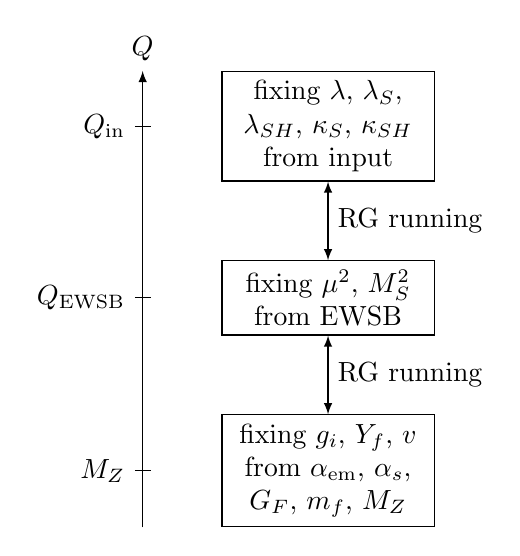
\begin{tikzpicture}
      \pgfmathsetmacro{\Qdist}{1};
      \node[block] (LowScaleInput) { fixing $g_i$, $Y_f$, $v$ from $\alpha_{\text{em}}$, $\alpha_s$, $G_F$, $m_f$, $M_Z$ };
      \node[block,above=1cm of LowScaleInput] (SUSYScaleInput) { fixing $\mu^2$, $M_S^2$ from EWSB };
      \node[block,above=1cm of SUSYScaleInput] (HighScaleInput) { fixing $\lambda$, $\lambda_S$, $\lambda_{SH}$, $\kappa_S$, $\kappa_{SH}$ from input };
      %
      \draw[<->] (LowScaleInput) -- node[right] {RG running} (SUSYScaleInput);
      \draw[<->] (SUSYScaleInput) -- node[right] {RG running} (HighScaleInput);
      \draw[->] ($(LowScaleInput.south west)+(-\Qdist,0)$) -- ($(HighScaleInput.north west)+(-\Qdist,0)$) node[above] {$Q$};
      \draw[] ($(LowScaleInput.west)+(-1.1*\Qdist,0)$) node[left] {$M_Z$} -- ($(LowScaleInput.west)+(-0.9*\Qdist,0)$);
      \draw[] ($(SUSYScaleInput.west)+(-1.1*\Qdist,0)$) node[left] {$Q_{\text{EWSB}}$} -- ($(SUSYScaleInput.west)+(-0.9*\Qdist,0)$);
      \draw[] ($(HighScaleInput.west)+(-1.1*\Qdist,0)$) node[left] {$Q_{\text{in}}$} -- ($(HighScaleInput.west)+(-0.9*\Qdist,0)$);
    \end{tikzpicture}
  \end{center}
\end{frame}

%%%%%%%%%%%%%%%%%%%%%%%%%%%%%%%%%%%%%%%%%%%%%%%%%%

\begin{frame}[fragile]{\insertsection\ -- FlexibleSUSY -- model file}
  Now we turn to create a \FlexibleSUSY\ model file.

  \bigskip

  1. Go to the \FlexibleSUSY\ directory:
  %
  \begin{lstlisting}
$ cd ~/hep-software/FlexibleSUSY-2.8.0\end{lstlisting}%$
  %
  Copy the SM model to a new model directory named \texttt{model\_files/SESM}
  %
  \begin{lstlisting}
$ mkdir -p model_files/SESM
$ cp model_files/SM/FlexibleSUSY.m.in \
    model_files/SESM/
$ cp model_files/SM/LesHouches.in.SM \
     model_files/SESM/LesHouches.in.SESM\end{lstlisting}%$
\end{frame}

%%%%%%%%%%%%%%%%%%%%%%%%%%%%%%%%%%%%%%%%%%%%%%%%%%

\begin{frame}[fragile]{\insertsection\ -- FlexibleSUSY -- model file}
  2. Edit the \FlexibleSUSY\ model file
  \texttt{model\_files/SESM/FlexibleSUSY.m.in}

  \bigskip

  Define new input parameters and the SLHA blocks they are read from:
  %
  \begin{lstlisting}
FSDefaultSARAHModel = SESM; (* SARAH model *)

MINPAR = {};

EXTPAR = {
    {0, Qin},
    {1, QEWSB},
    {2, LambdaIN},
    {3, LamSIN},
    {4, LamSHIN},
    {5, KapSIN},
    {6, KapSHIN},
    {7, vSIN}
};\end{lstlisting}%$
\end{frame}

%%%%%%%%%%%%%%%%%%%%%%%%%%%%%%%%%%%%%%%%%%%%%%%%%%

\begin{frame}[fragile]{\insertsection\ -- FlexibleSUSY -- model file}
  2. \ldots\ continuing \ldots

  \bigskip

  Fix the new parameters at appropriate scales by EWSB and by the
  input values:
  %
  \begin{lstlisting}
EWSBOutputParameters = { mu2, MS2 };

HighScaleInput = {
    {\[Lambda], LambdaIN},
    {LamS, LamSIN},
    {LamSH, LamSHIN},
    {KapS, KapSIN},
    {KapSH, KapSHIN}
};

SUSYScaleInput = {
    {vS, vSIN}
};\end{lstlisting}%$
\end{frame}

%%%%%%%%%%%%%%%%%%%%%%%%%%%%%%%%%%%%%%%%%%%%%%%%%%

\begin{frame}[fragile]{\insertsection\ -- FlexibleSUSY -- build}
  3. Create, configure and compile the FlexibleSUSY spectrum
  generator:
  %
  \begin{lstlisting}
$ LT=$HOME/hep-software/LoopTools/build

$ ./createmodel -f --name=SESM

$ ./configure --with-models=SESM \
     --with-loop-libraries=looptools \
     --with-looptools-incdir=${LT} \
     --with-looptools-libdir=${LT}

$ make -j4\end{lstlisting}%$
\end{frame}

%%%%%%%%%%%%%%%%%%%%%%%%%%%%%%%%%%%%%%%%%%%%%%%%%%

\begin{frame}[fragile]{\insertsection\ -- FlexibleSUSY -- SLHA input}
  4. Set reasonable values for the input parameters in the SLHA input
  file \texttt{model\_files/SESM/LesHouches.in.SESM}
  %
  \begin{lstlisting}
Block EXTPAR      # Input parameters
    0   1000      # input scale Qin
    1   173.34    # scale QEWSB
    2   0.21      # LambdaIN
    3   0.1       # LamSIN
    4   0.1       # LamSHIN
    5   100       # KapSIN
    6  -100       # KapSHIN
    7   3         # vSIN\end{lstlisting}%$
\end{frame}

%%%%%%%%%%%%%%%%%%%%%%%%%%%%%%%%%%%%%%%%%%%%%%%%%%

\begin{frame}[fragile]{\insertsection\ -- FlexibleSUSY -- run}
  5. Run FlexibleSUSY:
  %
  \begin{lstlisting}
$ models/SESM/run_SESM.x \
    --slha-input-file=model_files/SESM/LesHouches.in.SESM\end{lstlisting}%$
\end{frame}

%%%%%%%%%%%%%%%%%%%%%%%%%%%%%%%%%%%%%%%%%%%%%%%%%%

\subsection{SPheno}

%%%%%%%%%%%%%%%%%%%%%%%%%%%%%%%%%%%%%%%%%%%%%%%%%%

\begin{frame}{Table of Contents}
  \tableofcontents[currentsection,currentsubsection]
\end{frame}

%%%%%%%%%%%%%%%%%%%%%%%%%%%%%%%%%%%%%%%%%%%%%%%%%%

\begin{frame}[fragile]{\insertsection\ -- SPheno -- model file}
  Finally, let's create a \SPheno\ spectrum generator.

  \bigskip

  1. Go to the \SARAH\ directory and copy the model file
  \texttt{SPheno.m} from the SM to the SESM model directory:
  %
  \begin{lstlisting}
$ cd ~/hep-software/SARAH
$ cp Models/SM/SPheno.m Models/SESM/\end{lstlisting}%$
\end{frame}

%%%%%%%%%%%%%%%%%%%%%%%%%%%%%%%%%%%%%%%%%%%%%%%%%%

\begin{frame}[fragile]{\insertsection\ -- SPheno -- model file}
  2. Modify the \texttt{SPheno.m} model file to define new input
  parameters:
  %
  \begin{lstlisting}
MINPAR = {
    {2, LambdaIN},
    {3, LambdaSIN},
    {4, LambdaSHIN},
    {5, KappaSIN},
    {6, KappaSHIN},
    {7, vevSIN}
};\end{lstlisting}%$
\end{frame}

%%%%%%%%%%%%%%%%%%%%%%%%%%%%%%%%%%%%%%%%%%%%%%%%%%

\begin{frame}[fragile]{\insertsection\ -- SPheno -- model file}
  2. \ldots\ continuing \ldots

  \bigskip

  Fix the new parameters by EWSB and the input values :
  %
  \begin{lstlisting}
ParametersToSolveTadpoles = {mu2, MS2};

BoundaryLowScaleInput = {
    {\[Lambda], LambdaIN},
    {LambdaS, LambdaSIN},
    {LambdaSH, LambdaSHIN},
    {KapS, KappaSIN},
    {KapSH, KappaSHIN},
    {vS, vevSIN}
};\end{lstlisting}%$
\end{frame}

%%%%%%%%%%%%%%%%%%%%%%%%%%%%%%%%%%%%%%%%%%%%%%%%%%

\begin{frame}[fragile]{\insertsection\ -- SPheno -- model file}
  3. Create the FORTRAN files for the \SPheno\ spectrum generator:
  %
  \begin{lstlisting}
$ math
In[]:= << SARAH`
In[]:= Start["SESM"]
In[]:= MakeSPheno[]
In[]:= Quit[]'\end{lstlisting}%$
\end{frame}

%%%%%%%%%%%%%%%%%%%%%%%%%%%%%%%%%%%%%%%%%%%%%%%%%%

\begin{frame}[fragile]{\insertsection\ -- SPheno -- model file}
  4. Go to the \SPheno\ directory:
  %
  \begin{lstlisting}
$ cd ~/hep-software/SPheno-4.0.5\end{lstlisting}%$
  %
  Copy the generated FORTRAN files from the \SARAH\ directory to the
  \SPheno\ directory and compile the spectrum generator:
  %
  \begin{lstlisting}
$ mv ~/hep-software/SARAH/Output/SESM/EWSB/SPheno SESM
$ make F90=gfortran
$ make F90=gfortran Model=SESM\end{lstlisting}%$
\end{frame}

%%%%%%%%%%%%%%%%%%%%%%%%%%%%%%%%%%%%%%%%%%%%%%%%%%

\begin{frame}[fragile]{\insertsection\ -- SPheno -- model file}
  5. Set the input parameters to reasonable values in the SLHA input
  file \texttt{SESM/Input\_Files/LesHouches.in.SESM}:
  %
  \begin{lstlisting}
Block MINPAR   # Input parameters 
 2   0.21      # LambdaIN
 3   0.1       # LamSIN
 4   0.1       # LamSHIN
 5   100       # KapSIN
 6  -100       # KapSHIN
 7   3         # vSIN\end{lstlisting}%$
  %
  6. Run the \SPheno\ spectrum generator:
  \begin{lstlisting}
$ ./bin/SPhenoSSM \
     SESM/Input_Files/LesHouches.in.SESM\end{lstlisting}%$
  and inspect the output:
  \begin{lstlisting}
$ less SPheno.spc.SESM\end{lstlisting}%$
\end{frame}

%%%%%%%%%%%%%%%%%%%%%%%%%%%%%%%%%%%%%%%%%%%%%%%%%%

\section{Standard Model + S + S}

%%%%%%%%%%%%%%%%%%%%%%%%%%%%%%%%%%%%%%%%%%%%%%%%%%

\begin{frame}{Table of Contents}
  \tableofcontents[currentsection]
\end{frame}

%%%%%%%%%%%%%%%%%%%%%%%%%%%%%%%%%%%%%%%%%%%%%%%%%%

\begin{frame}{\insertsection}
  As a second example, let us consider an extension of the SESM by
  another real scalar gauge singlet. The model should be called Two
  Singlet Extension of the Standard Model (\TSESM). The Lagrangian
  should have a global $Z_2$ symmetry with all non-SESM fields having
  $Z_2$ charge $-1$:
  %
  \begin{equation*}
    \Lagr_{\TSESM} = \Lagr_{\SESM} - \left[\frac{\tilde\lambda_{SH}}{2} H^\dagger H \tilde{s}^2 + \frac{\tilde{M}_S^2}{2} \tilde{s}^2 + \frac{\tilde{\lambda}_S}{2} \tilde{s}^4\right]
  \end{equation*}
  %
  We will proceed as follows:
  %
  \begin{enumerate}
  \item Create a \SARAH\ model file for the TSESM
  \item Create a \FlexibleSUSY\ model file for the TSESM
  \item Create a \micrOMEGAs\ model file for the TSESM
  \item Run \FlexibleSUSY\ and pass the output to \micrOMEGAs\ to
    calculate the dark matter relic abundance $\Omega h^2$ etc.
  \end{enumerate}
\end{frame}

%%%%%%%%%%%%%%%%%%%%%%%%%%%%%%%%%%%%%%%%%%%%%%%%%%

\subsection{SARAH}

%%%%%%%%%%%%%%%%%%%%%%%%%%%%%%%%%%%%%%%%%%%%%%%%%%

\begin{frame}{Table of Contents}
  \tableofcontents[currentsection,currentsubsection]
\end{frame}

%%%%%%%%%%%%%%%%%%%%%%%%%%%%%%%%%%%%%%%%%%%%%%%%%%

\begin{frame}[fragile]{\insertsection\ -- SARAH -- model file}
  First, we modify \texttt{Models/TSESM/TSESM.m}:

  \medskip

  1. Add a global $Z_2$ symmetry and assign the charge $+1$ to each SESM
  field:
  %
  \begin{lstlisting}
Global[[1]] = {Z[2], Z2};

Gauge[[1]]={..., 1};
Gauge[[2]]={..., 1};
Gauge[[3]]={..., 1};

FermionFields[[1]] = {..., 1};
FermionFields[[2]] = {..., 1};
FermionFields[[3]] = {..., 1};
FermionFields[[4]] = {..., 1};
FermionFields[[5]] = {..., 1};

ScalarFields[[1]] = {..., 1};
ScalarFields[[2]] = {..., 1};\end{lstlisting}
\end{frame}

%%%%%%%%%%%%%%%%%%%%%%%%%%%%%%%%%%%%%%%%%%%%%%%%%%

\begin{frame}[fragile]{\insertsection\ -- SARAH -- model file}
  %
  2. Add the new scalar field $\tilde{s}$ with $Z_2$ charge $-1$:
  %
  \begin{lstlisting}
ScalarFields[[3]] = {ts, 1, TSing, 0, 1, 1, -1};
RealScalars = {s, ts};\end{lstlisting}
  %
  3. Extend the Lagrangian:
  %
  \begin{lstlisting}
LagNoHC = -(
    ...
    + TLamSH/2 conj[H].H.ts.ts
    + TMS2/2 ts.ts
    + TLamS/2 ts.ts.ts.ts
);\end{lstlisting}
\end{frame}

%%%%%%%%%%%%%%%%%%%%%%%%%%%%%%%%%%%%%%%%%%%%%%%%%%

\begin{frame}[fragile]{\insertsection\ -- SARAH -- model file}
  4. Modify the particle information in
  \texttt{Models/TSESM/particles.m}.

  \bigskip

  First, define the new \texttt{TSing} EWSB eigenstate (= gauge eigenstate)
  %
  \begin{lstlisting}
ParticleDefinitions[EWSB] = {
  ...
  {TSing, { Description -> "Singlet",
            PDG -> {6666635},
            PDG.IX -> {101000002},
            FeynArtsNr -> 10,
            Mass -> LesHouches,
            LaTeX -> "\\tilde{s}",
            ElectricCharge -> 0,
            LHPC -> {"gold"},
            OutputName -> "ts" }}
};\end{lstlisting}
\end{frame}

%%%%%%%%%%%%%%%%%%%%%%%%%%%%%%%%%%%%%%%%%%%%%%%%%%

\begin{frame}[fragile]{\insertsection\ -- SARAH -- model file}
  5. Modify the parameter information in
  \texttt{Models/TSESM/parameters.m}.

  \bigskip

  Add the new model parameters and their properties
  %
  \begin{lstlisting}
ParameterDefinitions = {
  ...
  {TMS2, { Description -> "Singlet mass term",
           LaTeX -> "\\tilde{M}_{S}^2",
           Real -> True, 
           OutputName -> TMS2,
           LesHouches -> {HMIX,35} }}, 

  {TLamSH, { OutputName -> TLamSH,
             LaTeX -> "\\tilde{\\lambda}_{SH}",
             Real -> True, 
             LesHouches -> {HMIX,36} }},
  ...
};\end{lstlisting}
\end{frame}

%%%%%%%%%%%%%%%%%%%%%%%%%%%%%%%%%%%%%%%%%%%%%%%%%%

\begin{frame}[fragile]{\insertsection\ -- SARAH -- model file}
  5. \ldots\ continuing \ldots
  %
  \begin{lstlisting}
ParameterDefinitions = {
  ...
  {TLamS, { OutputName -> TLamS,
            LaTeX -> "\\tilde{\\lambda}_{S}",
            Real -> True, 
            LesHouches -> {HMIX,37} }}
};\end{lstlisting}
\end{frame}

%%%%%%%%%%%%%%%%%%%%%%%%%%%%%%%%%%%%%%%%%%%%%%%%%%

\begin{frame}[fragile]{\insertsection\ -- SARAH -- check model}
  6. Check the \SARAH\ model
  %
  \begin{lstlisting}
$ math
In[]:= << SARAH`
In[]:= Start["TSESM"]
In[]:= CheckModel[]
In[]:= Quit[]'\end{lstlisting}%$
\end{frame}

%%%%%%%%%%%%%%%%%%%%%%%%%%%%%%%%%%%%%%%%%%%%%%%%%%

\subsection{FlexibleSUSY}

%%%%%%%%%%%%%%%%%%%%%%%%%%%%%%%%%%%%%%%%%%%%%%%%%%

\begin{frame}{Table of Contents}
  \tableofcontents[currentsection,currentsubsection]
\end{frame}

%%%%%%%%%%%%%%%%%%%%%%%%%%%%%%%%%%%%%%%%%%%%%%%%%%

\begin{frame}[fragile]{\insertsection\ -- FlexibleSUSY -- model file}
  Now we create a \FlexibleSUSY\ model file for the TSESM.

  \bigskip

  1. Go to the \FlexibleSUSY\ directory:
  %
  \begin{lstlisting}
$ cd ~/hep-software/FlexibleSUSY-2.8.0\end{lstlisting}%$
  %
  Copy the SESM model to a new model directory named
  \texttt{model\_files/TSESM}
  %
  \begin{lstlisting}
$ mkdir -p model_files/TSESM
$ cp model_files/SESM/FlexibleSUSY.m.in \
    model_files/TSESM/
$ cp model_files/SESM/LesHouches.in.SM \
     model_files/TSESM/LesHouches.in.TSESM\end{lstlisting}%$
\end{frame}

%%%%%%%%%%%%%%%%%%%%%%%%%%%%%%%%%%%%%%%%%%%%%%%%%%

\begin{frame}[fragile]{\insertsection\ -- FlexibleSUSY -- model file}
  2. Edit the \FlexibleSUSY\ model file
  \texttt{model\_files/TSESM/FlexibleSUSY.m.in}

  \bigskip

  Define new input parameters and the SLHA blocks they are read from
  and set the new parameters to their input value:
  %
  \begin{lstlisting}
FSDefaultSARAHModel = TSESM; (* SARAH model *)

EXTPAR = {
    ...
    {8, TLamSIN},
    {9, TLamSHIN},
    {10, TMS2IN}
};

HighScaleInput = {
    ...
    {TLamS, TLamSIN},
    {TLamSH, TLamSHIN},
    {TMS2, TMS2IN}
};\end{lstlisting}%$
\end{frame}

%%%%%%%%%%%%%%%%%%%%%%%%%%%%%%%%%%%%%%%%%%%%%%%%%%

\begin{frame}[fragile]{\insertsection\ -- FlexibleSUSY -- build}
  3. Create, configure and compile the FlexibleSUSY spectrum
  generator:
  %
  \begin{lstlisting}
$ LT=$HOME/hep-software/LoopTools/build

$ ./createmodel -f --name=TSESM

$ ./configure --with-models=TSESM \
     --with-loop-libraries=looptools \
     --with-looptools-incdir=${LT} \
     --with-looptools-libdir=${LT}

$ make -j4\end{lstlisting}%$
\end{frame}

%%%%%%%%%%%%%%%%%%%%%%%%%%%%%%%%%%%%%%%%%%%%%%%%%%

\begin{frame}[fragile]{\insertsection\ -- FlexibleSUSY -- SLHA input}
  4. Set reasonable values for the new input parameters in the SLHA
  input file \texttt{model\_files/TSESM/LesHouches.in.TSESM}
  %
  \begin{lstlisting}
Block EXTPAR      # Input parameters
    ...
    8   0.1       # TLamSIN
    9   0.1       # TLamSHIN
   10   1e3       # TMS2IN\end{lstlisting}%$
\end{frame}

%%%%%%%%%%%%%%%%%%%%%%%%%%%%%%%%%%%%%%%%%%%%%%%%%%

\begin{frame}[fragile]{\insertsection\ -- FlexibleSUSY -- run}
  5. Run FlexibleSUSY:
  %
  \begin{lstlisting}
$ models/TSESM/run_TSESM.x \
    --slha-input-file=model_files/TSESM/LesHouches.in.TSESM\end{lstlisting}%$
  %
  Predicted Higgs masses from the output:
  %
  \begin{lstlisting}
Block MASS
   6666635     6.18452698E+01   # TSing
        25     1.23989800E+02   # hh(1)
        35     6.90311044E+02   # hh(2)\end{lstlisting}
\end{frame}

%%%%%%%%%%%%%%%%%%%%%%%%%%%%%%%%%%%%%%%%%%%%%%%%%%

\subsection{micrOMEGAs}

%%%%%%%%%%%%%%%%%%%%%%%%%%%%%%%%%%%%%%%%%%%%%%%%%%

\begin{frame}{Table of Contents}
  \tableofcontents[currentsection,currentsubsection]
\end{frame}

%%%%%%%%%%%%%%%%%%%%%%%%%%%%%%%%%%%%%%%%%%%%%%%%%%

\begin{frame}[fragile]{\insertsection\ -- FlexibleSUSY -- run}
  Our plan is now to pass the \FlexibleSUSY\ output to \micrOMEGAs.

  \medskip

  1. In order to setup \micrOMEGAs\ for the TSESM, we need to first
  generate appropriate \micrOMEGAs/\CalcHEP\ model files with \SARAH:
  %
  \begin{lstlisting}
$ cd ~/hep-software/SARAH
$ math
In[]:= << SARAH`
In[]:= Start["TSESM"]
In[]:= MakeCHep[DMcandidate1 -> Z2 == -1, IncludeEffectiveHiggsVertices -> False]
In[]:= Quit[]\end{lstlisting}%$
\end{frame}

%%%%%%%%%%%%%%%%%%%%%%%%%%%%%%%%%%%%%%%%%%%%%%%%%%

\begin{frame}[fragile]{\insertsection\ -- FlexibleSUSY -- run}
  2. We go to the \micrOMEGAs\ directory and setup the new TSESM
  model:
  %
  \begin{lstlisting}
$ cd ~/hep-software/micromegas_6.1.15
$ ./newProject TSESM
$ cd TSESM
$ cp ~/hep-software/SARAH/Output/TSESM/EWSB/CHep/* work/models/
$ make main=main.cpp\end{lstlisting}%$
\end{frame}

%%%%%%%%%%%%%%%%%%%%%%%%%%%%%%%%%%%%%%%%%%%%%%%%%%

\begin{frame}[fragile]{\insertsection\ -- FlexibleSUSY -- run}
  3. We run FlexibleSUSY and place the SLHA output in the current
  directory with the name \texttt{SPheno.spc.TSESM}
  %
  \begin{lstlisting}
$ FS=$HOME/hep-software/FlexibleSUSY-2.8.0

$ ${FS}/models/TSESM/run_TSESM.x \
     --slha-input-file=${FS}/model_files/TSESM/LesHouches.in.TSESM \
     > SPheno.spc.TSESM\end{lstlisting}%$
  %
  4. We run \micrOMEGAs:
  %
  \begin{lstlisting}
$ ./main data.par\end{lstlisting}%$
\end{frame}

\end{document}
